\documentclass[10pt,a4paper]{article}
\usepackage[margin=2cm]{geometry}
\usepackage{amsmath,amssymb,booktabs,graphicx,caption,xcolor,float,hyperref,tikz}
\usetikzlibrary{arrows.meta,positioning,calc}
\hypersetup{colorlinks=true,linkcolor=blue!50!black,urlcolor=blue!50!black}
\captionsetup{font=small,labelfont=bf}
\title{\vspace{-1.2cm}\textbf{Steering a swarm that owns a proof}\\[2pt]
\large Simulation 2 (asynchronous activation), setup \texttt{task003-symmetric}}
\author{LLM-free simulator; report of 15 October 2026; runs of 15 October 2026\\
\small Mirrors the Simulation 1 report of the same date: same sections, figures and equations.}
\date{}
\begin{document}
\maketitle
\vspace{-1cm}

\paragraph{How the simulator works.} The world, \texttt{task\_003}, has three candidate allocations; A0 is the
correct one. Each of 24 agents is given one true fact and reasons as an exact Bayesian: its \emph{belief} is the
exact probability of A0, A1 and A2 given the facts it currently remembers. There are no rounds. Each agent acts
at random times, on average once per time unit: it reads $q$ posts drawn at random from the 48 most recent posts
on a shared \emph{board} (never its own), adds their facts to its memory, recomputes its belief, \emph{votes} by
probability matching (a vote drawn from its belief) and posts one remembered fact that supports its vote. Every
remembered fact is forgotten after a random lifetime (on average a fraction $\rho$ survives one time unit; reading
it again renews it). A \emph{controller} with a target, A0 (truth) or A2 (false), acts at random times at rate
$\lambda_c$ until $t = 30$: it reads $q_c$ recent agent posts and, unless the \emph{vote gate} (at least 75\% of
them from agents voting for its target) or the \emph{proof stop} (its target already proved) silences it, posts
the one fact from its pool that best supports its target, at most 30 messages per episode. Agents continue
alone until $t = 40$. Every episode is run three times with the same random draws: without a controller
(\emph{silent}), with the controller targeting A0 and with the one targeting A2.

\paragraph{The facts at the start.} All facts are true. The agents hold, together, a proof of A0; no single
agent does, and neither pool can prove its target (Table~\ref{tab:facts}).

\begin{table}[H]
\centering\small
\caption{Facts available at $t = 0$ and what each set implies, $P(\text{A0}, \text{A1}, \text{A2} \mid \text{facts})$.}
\label{tab:facts}
\begin{tabular}{lcc}
\toprule
set of facts & facts & $P(\text{A0}, \text{A1}, \text{A2})$ \\
\midrule
agents' facts, all together (24 agents, one fact each) & 18 distinct & (1, 0, 0): proves A0 \\
A0 pool (controller with target A0) & 12, of which 10 new to the agents & (0.963, 0.037, 0) \\
A2 pool (controller with target A2) & 12, of which 10 new to the agents & (0.114, 0, 0.886) \\
agents' facts + either pool & 28 distinct & (1, 0, 0) \\
\bottomrule
\end{tabular}
\end{table}

\paragraph{The runs.} Posts read by an agent $q \in \{3, 6, 12\}$; posts read by the controller
$q_c \in \{3, 6, 12, 24\}$; controller rate $\lambda_c \in \{0.5, 1, 2, 3, 4, 5, 6, 7, 8\}$ (one fact per
message); memory $\rho \in \{1, 0.75, 0.5, 0.25\}$; vote gate on and off; proof stop on; 1{,}000 episodes per
setting (1{,}740 settings). Unless stated otherwise: $q = 6$, $q_c = 12$, $\lambda_c = 1$ (the main setting,
which posts about as many facts as Simulation 1 with one fact per night), gate on. Gate-off results are in
Appendix~\ref{app:gateoff}.

\paragraph{Summary.} The 24 agents together own a proof of A0, and with full memory they keep it: no controller
changes the swarm for more than a few time units. \textbf{Forgetting is what makes the swarm steerable}, and in this
simulation the shorter the memory, the larger the effect: at $t = 30$ the false controller raises the share voting A2
by 0.09--0.15 ($\rho = 0.75$), 0.27--0.37 ($\rho = 0.5$) and 0.37--0.44 ($\rho = 0.25$), and wins the majority when
$\rho \le 0.5$ (Figures~\ref{fig:votes}, \ref{fig:gaintime}). \textbf{The 30-message budget, not the rate, sets the
end point}: a faster controller only gets there sooner (at $t = 5$, $0.08 \to 0.39$ from the slowest to the fastest
rate; at $t = 30$ almost no gain beyond $\lambda_c = 1$), and the slowest controller is 1.6 to 4 times more
effective per fact (Figures~\ref{fig:strength}, \ref{fig:perfact}). \textbf{Reading more posts protects the proof
when agents remember, and helps the controller when they forget} (Figure~\ref{fig:phasegain}c). Every controller
replaces part of the agents' own proofs (Figure~\ref{fig:proofs}). The target is most readable at $\rho = 0.25$
(0.27--0.37 bits from one vote); the efficiency $\eta$ is 0.79--0.94 almost everywhere
(Figures~\ref{fig:Itime}--\ref{fig:phaseeta}). The vote gate matters little (Appendix~\ref{app:gateoff}). Swarm-level
states read up to nine times more than one vote, with a lower efficiency (Appendix~\ref{app:states}).

\section{Quantities}\label{sec:quantities}

\paragraph{Votes.} With $n_{a,t}$ the number of agents whose last vote is answer $a$ at time $t$ and $N_t$ the
number of agents who have voted,
\begin{equation}\label{eq:share}
x_{a,t} = n_{a,t}/N_t .
\end{equation}
At $t = 0$ nobody has voted and we set $x_{a,0} = 0$; all agents have voted by $t \approx 5$. (The 9--14 October reports divided by 24, which counted agents who had
not yet acted as voting against the target; this inflated the apparent rise of the shares and the apparent bias of
the controller's sensing at early times.)

\paragraph{Paired susceptibility.} Following \texttt{BLACKBOARD\_OBSERVABLES\_AND\_EFFICIENCIES} (\S3), for a
controller policy $\pi$ and an answer $a$,
\begin{equation}\label{eq:chi}
\chi^{(a)}_{\pi,t} \equiv G^{(a)}_t(\pi) = \mathbb E\bigl[x^{\pi}_{a,t} - x^{\rm base}_{a,t}\bigr],
\end{equation}
the mean over episodes of the difference between the controlled run and the silent run of the same episode. We
report it on the controller's own target: $G_t \equiv G^{(0)}_t(\pi^{+})$ for the controller targeting A0 and
$G_t \equiv G^{(2)}_t(\pi^{-})$ for the one targeting A2.

\paragraph{Target and state.} The target $Z \in \{\text{A0}, \text{A2}\}$ is drawn by a fair coin. The state $X$
of the swarm at time $t$ is one of:
\begin{itemize}\itemsep1pt
\item \textbf{one agent's vote} (main text): the vote of a randomly chosen agent, $X \in \{\text{A0},\text{A1},\text{A2}\}$;
\item \textbf{plurality}: the answer with the most votes among all last votes (a $k$-way tie gives $1/k$ to each);
\item \textbf{S1}: the agents' mean belief in A0, $m_{\text{A0}}$, cut at 0.33, 0.50 and 0.75 (4 values);
\item \textbf{S3}: $(m_{\text{A0}}, m_{\text{A2}})$, each cut into thirds of $[0, 1]$ (9 values, 6 reachable).
\end{itemize}
Each episode $e$ of arm $s$ (silent 0, target A0 $+$, target A2 $-$) gives a probability vector $y^{(e)}_s$ over
the values of $X$ (for one agent's vote, the episode's vote shares; for the others, a mark on one value), and
\begin{equation}\label{eq:P}
P_s(x) = \frac1E\sum_{e=1}^{E} y^{(e)}_s(x), \qquad E = 1000 .
\end{equation}

\paragraph{Readability and efficiency.} With $Q = \frac12(P_+ + P_-)$ and $\mathrm{KL}(p\Vert q) = \sum_x p(x)\log_2[p(x)/q(x)]$,
\begin{equation}\label{eq:I}
I(Z;X) = \tfrac12\,\mathrm{KL}(P_+\Vert Q) + \tfrac12\,\mathrm{KL}(P_-\Vert Q),
\end{equation}
the information the state carries about the target (at most 1 bit). The controllers' total change from silence
splits exactly into a directed and an undirected part,
\begin{equation}\label{eq:C}
C = \tfrac12\,\mathrm{KL}(P_+\Vert P_0) + \tfrac12\,\mathrm{KL}(P_-\Vert P_0) = I(Z;X) + \mathrm{KL}(Q\Vert P_0),
\end{equation}
and the efficiency is the directed share,
\begin{equation}\label{eq:eta}
\eta = I(Z;X)/C .
\end{equation}
Silence sometimes never shows a value of $X$ that a controller reaches, which would make $C$ infinite. Before
computing any KL, every arm's distribution therefore receives the same pseudo-count of $\alpha = 0.5$ episodes per
value of $X$ ($K$ values),
\begin{equation}\label{eq:smooth}
\tilde P_s(x) = \frac{E\,P_s(x) + \alpha}{E + \alpha K}.
\end{equation}
With $\alpha = 1$ instead, $\eta$ changes by at most 0.004 for one agent's vote and 0.06 for the other states; where
$C$ is finite without smoothing, by at most 0.014. $\eta$ is not defined when $C < 0.01$ bits (no measurable change);
such values are left blank. Equation~(\ref{eq:C}) holds in the data to $4\times10^{-15}$ bits.

\paragraph{Cost.} $F_t$ is the number of facts the controller has posted up to $t$ (mean per episode); the gain
per fact is $G_t/F_t$, and the marginal susceptibility is the slope between neighbouring rates,
\begin{equation}\label{eq:slope}
\frac{\Delta G}{\Delta\lambda_c} = \frac{G(\lambda_c^{(k+1)}) - G(\lambda_c^{(k)})}{\lambda_c^{(k+1)} - \lambda_c^{(k)}} .
\end{equation}

\section{Votes over time}

\begin{figure}[H]
\centering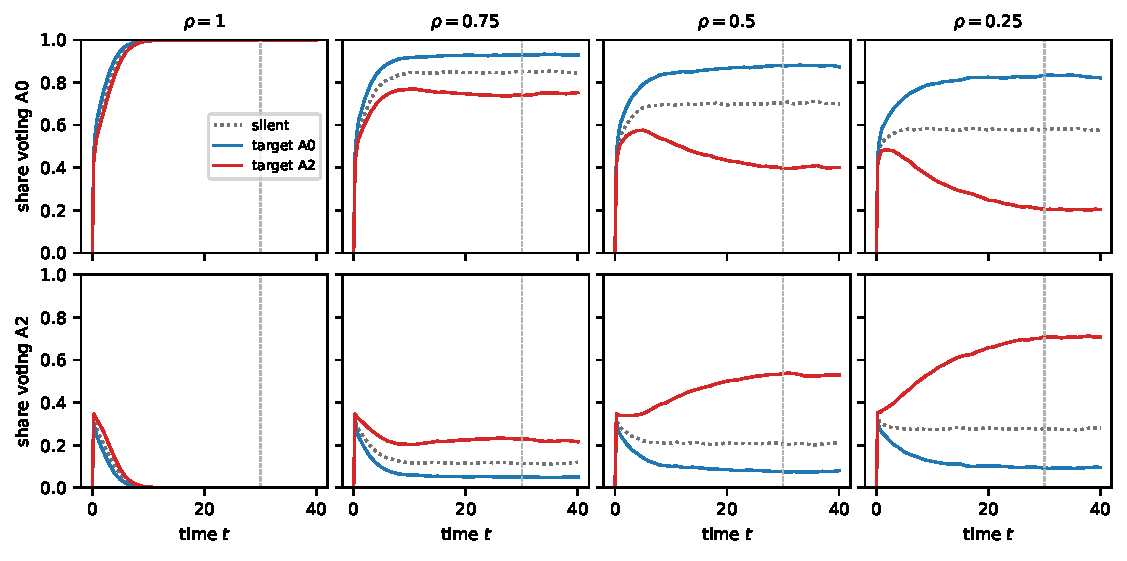
\includegraphics[width=0.95\linewidth]{figures/fig_votes.pdf}
\caption{Share of agents voting A0 (top) and A2 (bottom), Eq.~(\ref{eq:share}), without a controller (dotted),
with the controller targeting A0 (blue) and A2 (red); one column per memory $\rho$. $q = 6$, $q_c = 12$,
$\lambda_c = 1$, gate on. At $t = 0$ nobody has voted and every share is 0; after that the shares count only agents
who have voted (all have by $t \approx 5$). The controller stops at $t = 30$ (dashed). 95\% intervals are narrower
than the lines ($\pm 0.01$).}
\label{fig:votes}
\end{figure}

\begin{itemize}\itemsep1pt
\item \textbf{The shorter the memory, the less firmly the silent swarm holds the truth}: 100\%, 85\%, 71\% and
  58\% vote A0 at $t = 30$ for $\rho = 1, 0.75, 0.5, 0.25$.
\item \textbf{With full memory no controller matters}: every agent votes A0 by $t \approx 10$ in all three arms.
\item \textbf{The false controller wins the majority when $\rho \le 0.5$}: A2 gets 54\% ($\rho = 0.5$) and 71\%
  ($\rho = 0.25$) of the votes, against 21\% and 28\% in silence; at $\rho = 0.75$ only 23\%.
\item \textbf{The truth controller restores the truth} to 84--93\% at every $\rho < 1$.
\end{itemize}

\section{Paired susceptibility over time}

\begin{figure}[H]
\centering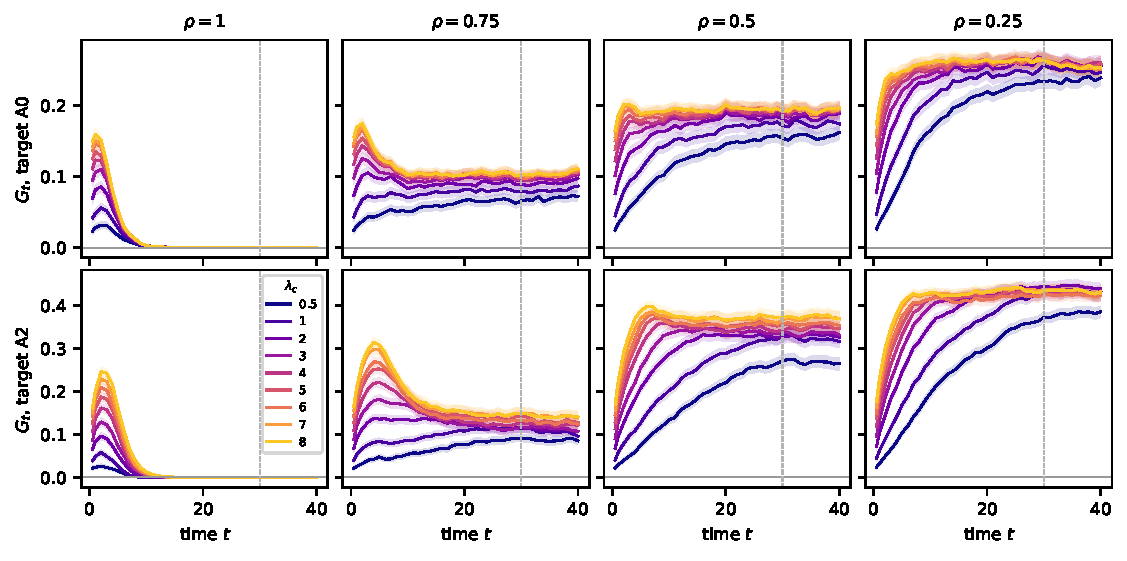
\includegraphics[width=0.95\linewidth]{figures/fig_gain_time.pdf}
\caption{Paired susceptibility $G_t$, Eq.~(\ref{eq:chi}), target A0 (top) and A2 (bottom), one curve per
controller rate $\lambda_c$; $q = 6$, $q_c = 12$, gate on. $G_0 = 0$: at $t = 0$ the three arms are identical.
Bands: 95\% intervals.}
\label{fig:gaintime}
\end{figure}

\begin{itemize}\itemsep1pt
\item \textbf{Susceptibility grows as memory shortens}: at $t = 30$, target A2, $G = 0.09$--$0.15$ ($\rho = 0.75$),
  $0.27$--$0.37$ ($\rho = 0.5$), $0.37$--$0.44$ ($\rho = 0.25$); target A0, $0.07$--$0.10$, $0.16$--$0.19$,
  $0.23$--$0.26$.
\item \textbf{With full memory control is only transient}: target A2 reaches $0.25$ at $t \approx 2$
  ($\lambda_c = 8$) and is gone by $t \approx 10$.
\item \textbf{Fast controllers overshoot when agents remember well}: at $\rho = 0.75$, target A2 with
  $\lambda_c = 8$ peaks at $0.32$ ($t \approx 4$) and relaxes to $0.15$; at $\rho \le 0.5$ the peak is kept.
\item \textbf{The effect persists after the controller stops}: from $t = 30$ to $40$, $G$ changes by at most
  $0.02$ in every setting of the figure.
\end{itemize}

\section{Phase diagrams of the susceptibility}

\begin{figure}[H]
\centering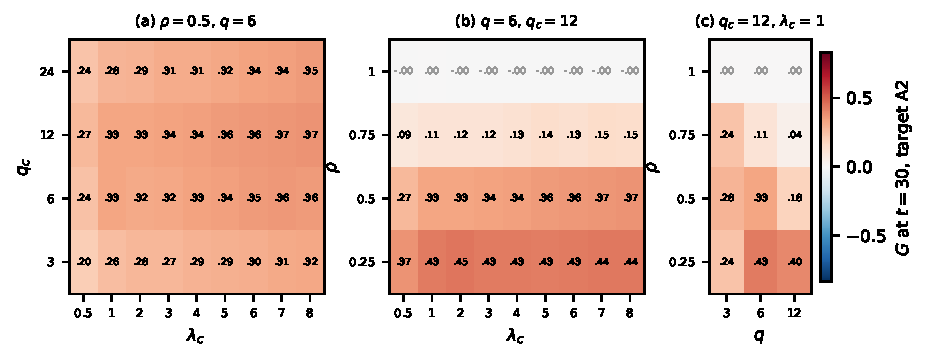
\includegraphics[width=0.98\linewidth]{figures/fig_phase_gain.pdf}
\caption{$G$ at $t = 30$, target A2, gate on: (a) over the posts the controller reads $q_c$ and its rate
$\lambda_c$, at $\rho = 0.5$, $q = 6$; (b) over $\rho$ and $\lambda_c$, at $q = 6$, $q_c = 12$; (c) over $\rho$
and the posts each agent reads $q$, at $q_c = 12$, $\lambda_c = 1$. Grey number: the 95\% interval includes 0.
Same colour scale as in the Simulation 1 report.}
\label{fig:phasegain}
\end{figure}

\begin{itemize}\itemsep1pt
\item \textbf{Memory is the main axis} (panel b): $G$ goes from 0 at $\rho = 1$ to $0.37$--$0.45$ at $\rho = 0.25$.
\item \textbf{The rate matters only up to $\lambda_c \approx 1$} (panels a, b): beyond it the 30-message budget is
  spent before $t = 30$.
\item \textbf{Reading more posts helps the controller slightly up to $q_c = 12$} (panel a: mean $G$ 0.28, 0.33,
  0.34, 0.31 for $q_c = 3, 6, 12, 24$).
\item \textbf{Reading more defends the proof only when agents remember well} (panel c): at $\rho = 0.75$, $G$
  falls from $0.24$ ($q = 3$) to $0.04$ ($q = 12$); at $\rho = 0.25$ it rises from $0.24$ to $0.40$--$0.43$
  ($q = 6$, 12). A likely reason, not tested: with heavy forgetting the proof cannot be rebuilt anyway, and
  reading more only spreads the controller's facts faster.
\end{itemize}

\section{Susceptibility against the rate, and its slope}

\begin{figure}[H]
\centering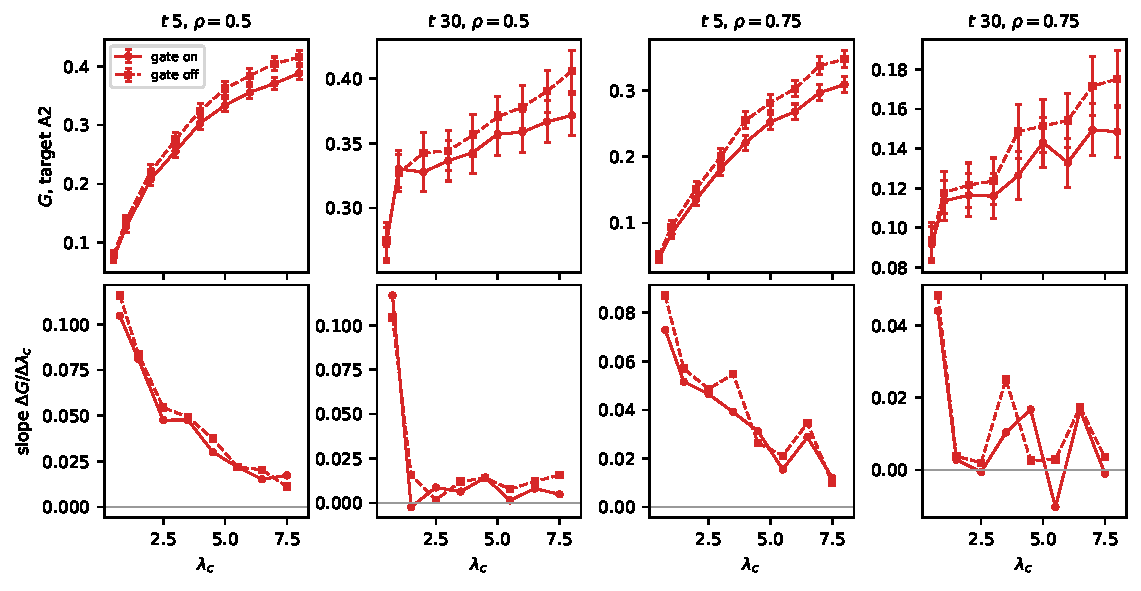
\includegraphics[width=0.95\linewidth]{figures/fig_gain_strength.pdf}
\caption{Top: $G$, target A2, against the controller rate $\lambda_c$, at $t = 5$ and $t = 30$ for $\rho = 0.5$
and $0.75$; gate on (solid) and off (dashed); bars: 95\% intervals. Bottom: the slope between neighbouring rates,
Eq.~(\ref{eq:slope}).}
\label{fig:strength}
\end{figure}

\begin{itemize}\itemsep1pt
\item \textbf{Early, speed buys susceptibility with steadily diminishing returns}: at $t = 5$, $\rho = 0.5$, $G$
  rises from $0.08$ ($\lambda_c = 0.5$) to $0.39$ ($\lambda_c = 8$); the slope falls from $0.11$ to about $0.02$
  per unit of rate.
\item \textbf{By $t = 30$ the slope is almost zero beyond $\lambda_c = 1$}: $0.12$ for the first step, $0.007$ on
  average after it ($\rho = 0.5$), because every fast controller has spent its 30 messages.
\item \textbf{The marginal susceptibility is the efficiency of adding rate}: high for the first unit of rate,
  close to zero after it once the decision has settled.
\item \textbf{Turning the gate off adds little}: at most $+0.03$ ($\rho = 0.5$, $t = 30$, $\lambda_c = 8$:
  $0.41$ against $0.37$).
\end{itemize}

\section{Susceptibility per fact posted}

\begin{figure}[H]
\centering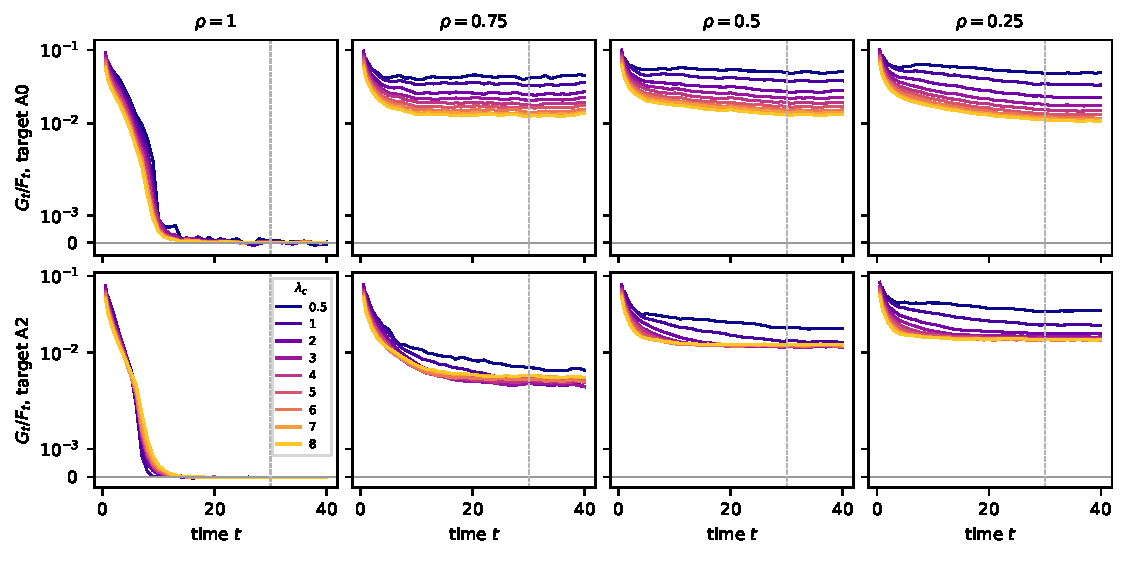
\includegraphics[width=0.95\linewidth]{figures/fig_gain_per_fact.pdf}
\caption{Gain per fact $G_t/F_t$ (log scale) for target A0 (top) and A2 (bottom), one curve per rate; $q = 6$,
$q_c = 12$, gate on. Shown once the controller has posted at least half a fact on average.}
\label{fig:perfact}
\end{figure}

\begin{itemize}\itemsep1pt
\item \textbf{The slowest controller gets the most per fact}: at $t = 30$, target A2, $\rho = 0.5$: $0.021$ per fact
  at $\lambda_c = 0.5$ (13 facts) against $0.013$ at $\lambda_c = 8$ (30 facts); at $\rho = 0.25$: $0.034$ against
  $0.015$.
\item \textbf{The truth controller gets more per fact than the false one} ($0.049$ against $0.021$ at $\rho = 0.5$,
  $\lambda_c = 0.5$): the gate keeps it silent once the swarm agrees, so it posts only 3--15 facts.
\item \textbf{Per fact, every controller is most effective in its first few time units} and declines as facts
  accumulate.
\end{itemize}

\section{Who holds the proof}

\begin{figure}[H]
\centering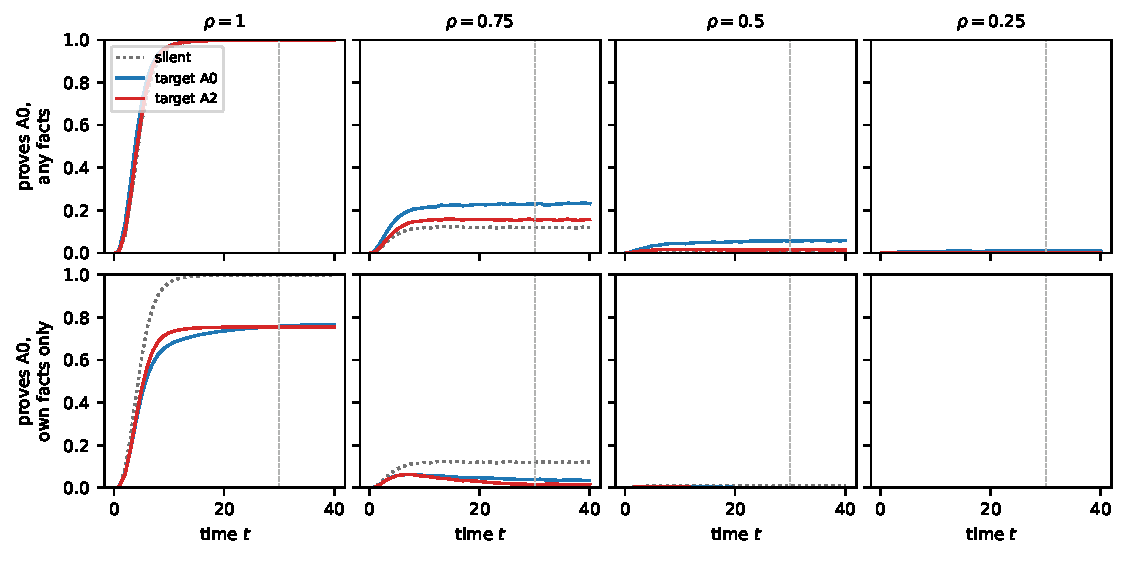
\includegraphics[width=0.95\linewidth]{figures/fig_proofs.pdf}
\caption{Share of agents whose remembered facts prove A0 (top) and prove it from the agents' original facts only
(bottom); silent (dotted), target A0 (blue), target A2 (red); $q = 6$, $q_c = 12$, $\lambda_c = 1$, gate on.}
\label{fig:proofs}
\end{figure}

\begin{itemize}\itemsep1pt
\item \textbf{Proofs need memory}: at $t = 30$ the silent swarm has 100\%, 12\%, 1\% and 0\% of agents proving A0
  for $\rho = 1, 0.75, 0.5, 0.25$. Below $\rho = 0.75$ votes rest on beliefs, not proofs.
\item \textbf{Every controller replaces the agents' own proofs}: with full memory all agents prove A0 under any
  arm, but only 76\% from their own facts under either controller (100\% in silence); at $\rho = 0.75$, 23\% prove A0
  under the truth controller but only 4\% from their own facts.
\item \textbf{The false controller's true facts complete proofs of A0} (16\% against 12\% in silence at
  $\rho = 0.75$).
\end{itemize}

\section{Readability over time}

\begin{figure}[H]
\centering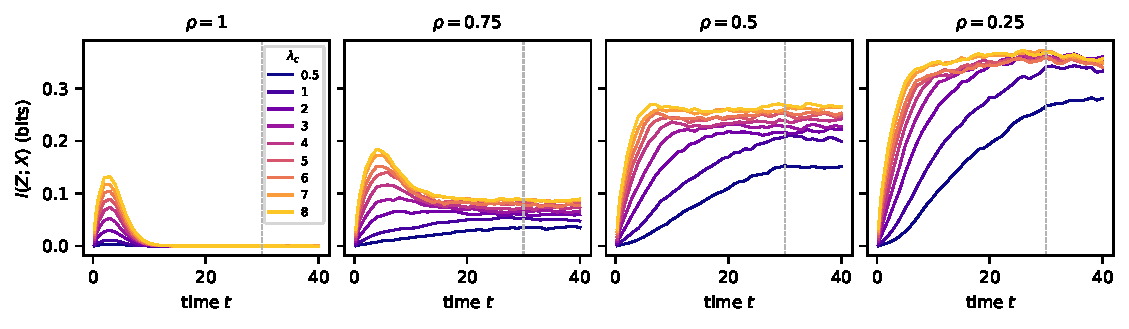
\includegraphics[width=0.95\linewidth]{figures/fig_I_time.pdf}
\caption{Readability $I(Z;X)$, Eq.~(\ref{eq:I}), with $X$ one agent's vote, one curve per rate; $q = 6$,
$q_c = 12$, gate on.}
\label{fig:Itime}
\end{figure}

\begin{itemize}\itemsep1pt
\item \textbf{The target is more readable when memory is shorter}: at $t = 30$, $I = 0.04$--$0.09$ bits
  ($\rho = 0.75$), $0.15$--$0.27$ ($\rho = 0.5$), $0.27$--$0.37$ ($\rho = 0.25$), 0 ($\rho = 1$).
\item \textbf{Fast controllers are readable early}: at $\rho = 0.75$ and $\lambda_c = 8$, $I$ peaks at $0.19$ bits
  ($t \approx 4$) and relaxes, as the susceptibility does.
\item \textbf{The rate orders the curves}: faster controllers are more readable at every $\rho < 1$.
\end{itemize}

\section{Efficiency over time}

\begin{figure}[H]
\centering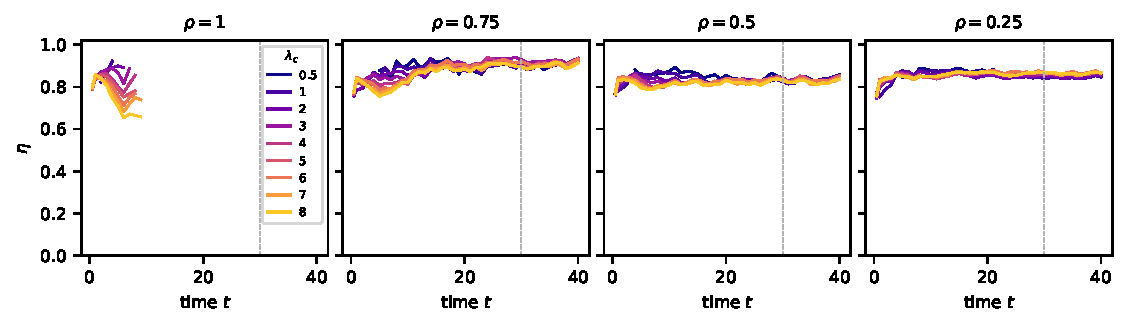
\includegraphics[width=0.95\linewidth]{figures/fig_eta_time.pdf}
\caption{Efficiency $\eta = I/C$, Eq.~(\ref{eq:eta}), one agent's vote, one curve per rate; $q = 6$, $q_c = 12$,
gate on. Blank: undefined ($C < 0.01$ bits). Pseudo-count, Eq.~(\ref{eq:smooth}).}
\label{fig:etatime}
\end{figure}

\begin{itemize}\itemsep1pt
\item \textbf{Efficiency is high and nearly flat}: at $t = 30$, $\eta = 0.89$--$0.93$ ($\rho = 0.75$),
  $0.82$--$0.84$ ($\rho = 0.5$), $0.84$--$0.87$ ($\rho = 0.25$).
\item \textbf{The rate barely changes it}: faster control raises $I$ and the total change $C$ together, so their
  ratio stays.
\item \textbf{With full memory $\eta$ is defined only early}, before the controllers' effects vanish.
\end{itemize}

\section{Phase diagrams of the readability}

\begin{figure}[H]
\centering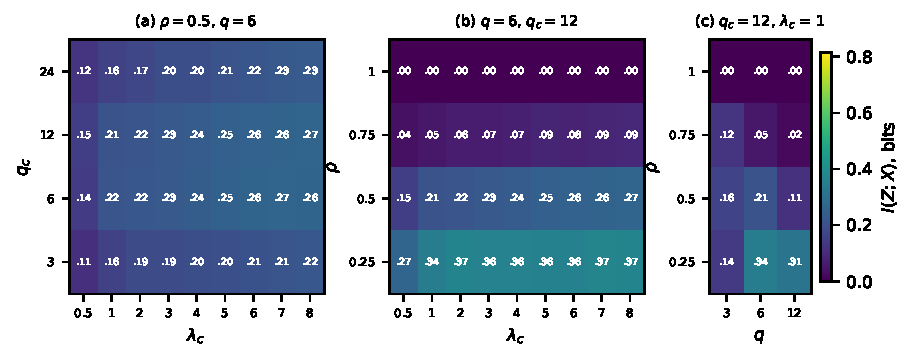
\includegraphics[width=0.98\linewidth]{figures/fig_phase_I.pdf}
\caption{$I(Z;X)$ at $t = 30$, one agent's vote, gate on; panels as in Figure~\ref{fig:phasegain}.}
\label{fig:phaseI}
\end{figure}

\begin{itemize}\itemsep1pt
\item \textbf{Readability follows the susceptibility}: lowest at $\rho = 0.75$ (0.04--0.09 bits), highest at
  $\rho = 0.25$ (up to 0.37); 0 at $\rho = 1$.
\item \textbf{The posts each agent reads have the same reversal as $G$} (panel c): at $\rho = 0.75$, $I$ falls from
  $0.12$ ($q = 3$) to $0.02$ ($q = 12$); at $\rho = 0.25$ it is $0.14$, $0.34$, $0.32$ for $q = 3, 6, 12$.
\item \textbf{$q_c$ and the rate change it by less than 0.15 bits} (panel a: 0.11--0.27).
\end{itemize}

\section{Phase diagrams of the efficiency}

\begin{figure}[H]
\centering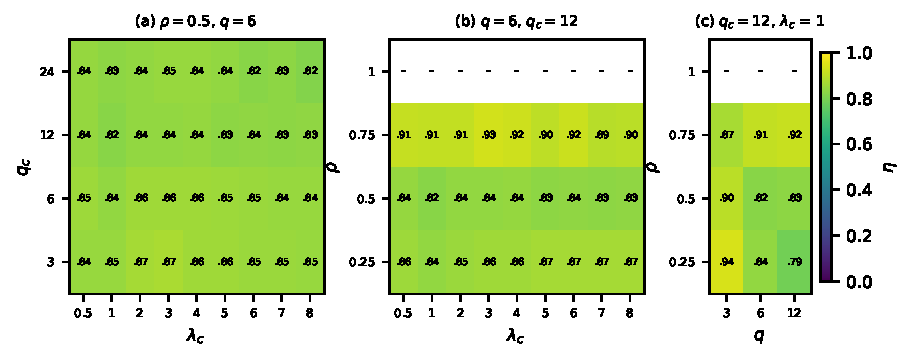
\includegraphics[width=0.98\linewidth]{figures/fig_phase_eta.pdf}
\caption{$\eta$ at $t = 30$, one agent's vote, gate on; panels as in Figure~\ref{fig:phasegain}. Dash: undefined.}
\label{fig:phaseeta}
\end{figure}

\begin{itemize}\itemsep1pt
\item \textbf{Efficiency is almost uniform}: 0.79--0.94 over every setting with $\rho < 1$.
\item \textbf{It is highest where the effects are smallest} ($\rho = 0.75$: 0.89--0.93): $\eta$ measures how
  mirror-like the two controllers' changes are, not how large they are; the size is $I$
  (Figure~\ref{fig:phaseI}).
\end{itemize}

\section{Conclusions}

\begin{enumerate}\itemsep2pt
\item \textbf{Memory decides whether a swarm that owns a proof can be steered.} With full memory every effect
  vanishes by $t \approx 10$. As memory shortens the silent swarm holds the truth less firmly (100\%, 85\%, 71\%,
  58\% voting A0 at $t = 30$) and the controllers' susceptibility rises steadily.
\item \textbf{The budget sets the end point; the rate sets the speed.} The marginal susceptibility of the rate is
  large early and close to zero by $t = 30$ beyond $\lambda_c = 1$; per fact, slow control is the most effective.
\item \textbf{Fast control overshoots when agents remember well} ($\rho = 0.75$: $0.32 \to 0.15$), and every effect
  persists after the controller stops (changes below 0.02 from $t = 30$ to 40).
\item \textbf{The posts each agent reads switch sides with memory}: they defend the proof at $\rho = 0.75$ and help
  the controller at $\rho = 0.25$.
\item \textbf{Control replaces the agents' own proofs}, even when every agent ends up proving the truth.
\item \textbf{Readability tracks susceptibility; efficiency is almost constant.} $I$ ranges from 0 to 0.37 bits;
  $\eta$ stays at 0.79--0.94 because the two controllers' effects scale together.
\item \textbf{Compared with Simulation 1} (same settings, about the same facts posted): Simulation 2 is less
  susceptible at $\rho = 0.5$ (0.33 against 0.53, target A2) and more at $\rho = 0.25$ (0.43 against 0.31), and its
  vote gate matters far less.
\end{enumerate}

\appendix
\section{Gate off}\label{app:gateoff}

\begin{figure}[H]
\centering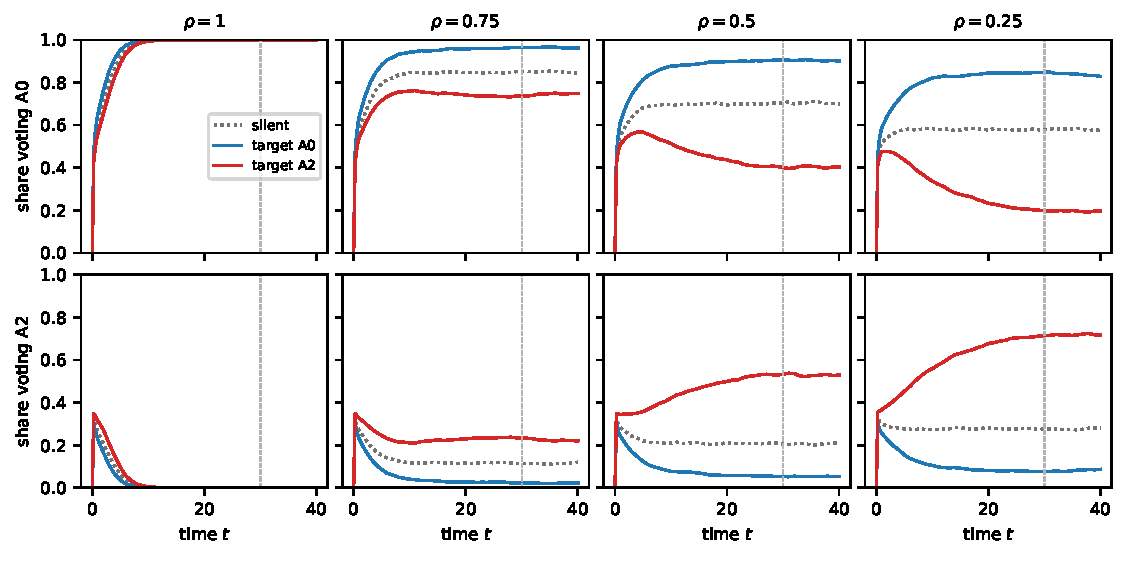
\includegraphics[width=0.95\linewidth]{figures/fig_votes_gateoff.pdf}
\caption{As Figure~\ref{fig:votes}, gate off.}
\label{fig:votesoff}
\end{figure}

\begin{figure}[H]
\centering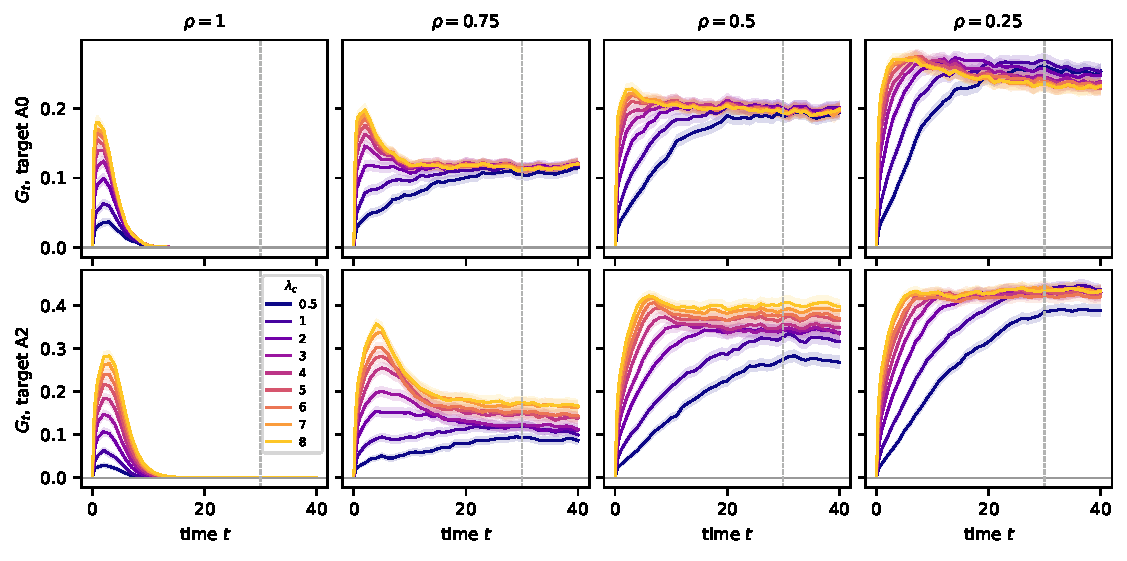
\includegraphics[width=0.95\linewidth]{figures/fig_gain_time_gateoff.pdf}
\caption{As Figure~\ref{fig:gaintime}, gate off.}
\label{fig:gaintimeoff}
\end{figure}

\begin{figure}[H]
\centering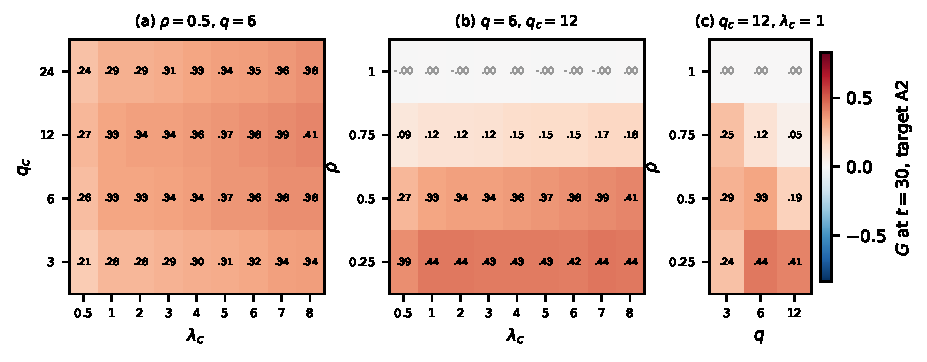
\includegraphics[width=0.98\linewidth]{figures/fig_phase_gain_gateoff.pdf}
\caption{As Figure~\ref{fig:phasegain}, gate off.}
\label{fig:phasegainoff}
\end{figure}

\begin{figure}[H]
\centering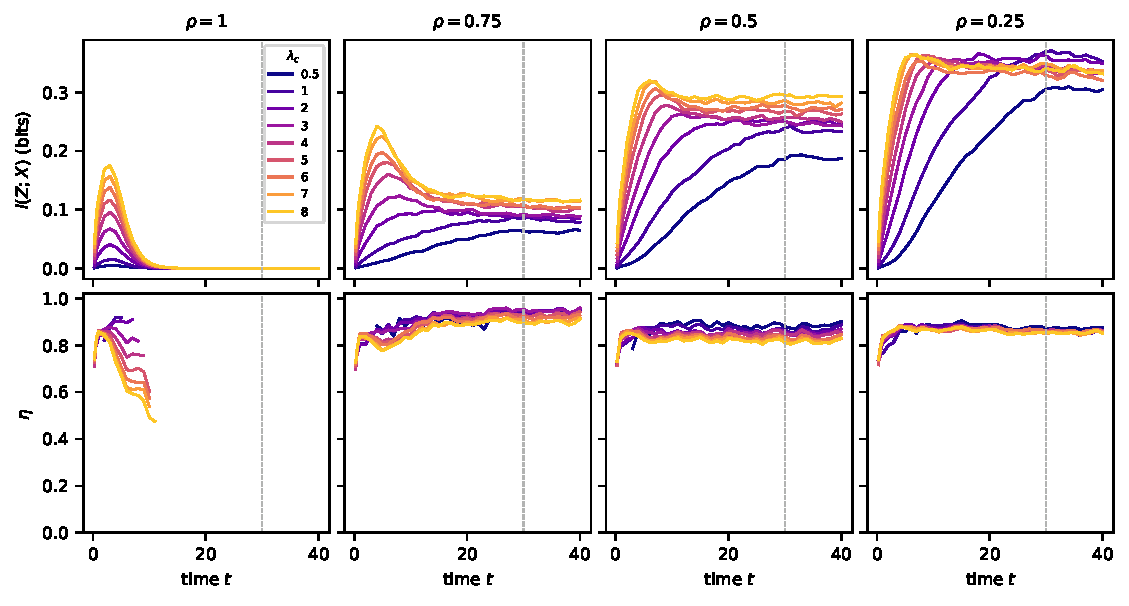
\includegraphics[width=0.95\linewidth]{figures/fig_Ieta_time_vote_gateoff.pdf}
\caption{As Figures~\ref{fig:Itime} (top) and \ref{fig:etatime} (bottom), gate off.}
\label{fig:infooff}
\end{figure}

\begin{figure}[H]
\centering
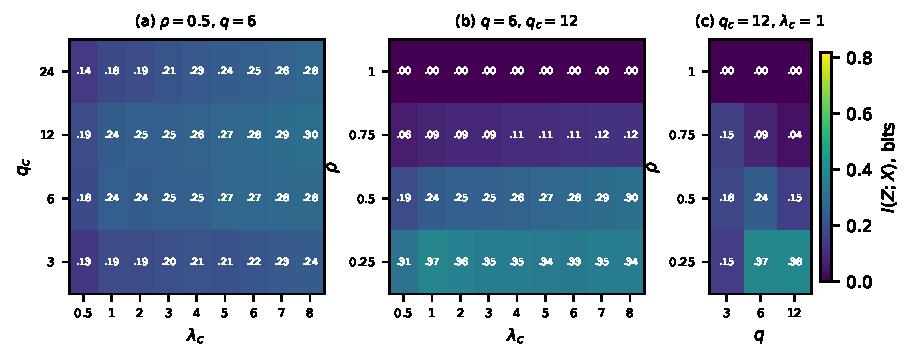
\includegraphics[width=0.98\linewidth]{figures/fig_phase_I_gateoff.pdf}\\
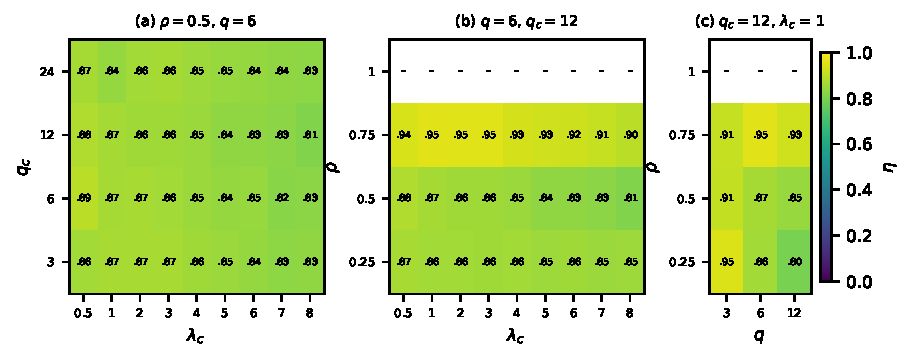
\includegraphics[width=0.98\linewidth]{figures/fig_phase_eta_gateoff.pdf}
\caption{As Figures~\ref{fig:phaseI} (top) and \ref{fig:phaseeta} (bottom), gate off.}
\label{fig:phaseinfooff}
\end{figure}

\begin{itemize}\itemsep1pt
\item \textbf{The gate matters little here}: at $t = 30$ turning it off changes $G$ by $-0.03$ to $+0.04$, $I$ by
  at most $0.03$ bits on average, $\eta$ by at most $0.02$.
\item \textbf{It mostly saves the truth controller's messages}: 11--23 more facts per episode with the gate off;
  the false controller is rarely gated (0--3 more).
\end{itemize}

\section{Other states}\label{app:states}

\begin{figure}[H]
\centering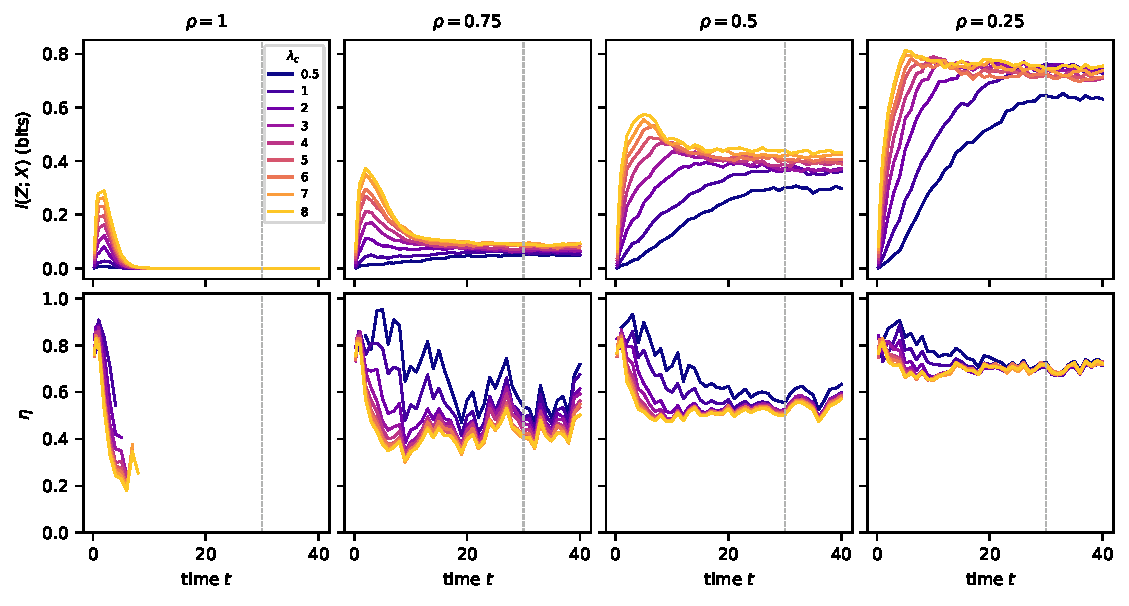
\includegraphics[width=0.95\linewidth]{figures/fig_Ieta_time_plur.pdf}
\caption{Readability (top) and efficiency (bottom) over time with $X$ = the plurality of the last votes; layout
as in Figures~\ref{fig:Itime} and \ref{fig:etatime}.}
\label{fig:plurtime}
\end{figure}

\begin{figure}[H]
\centering
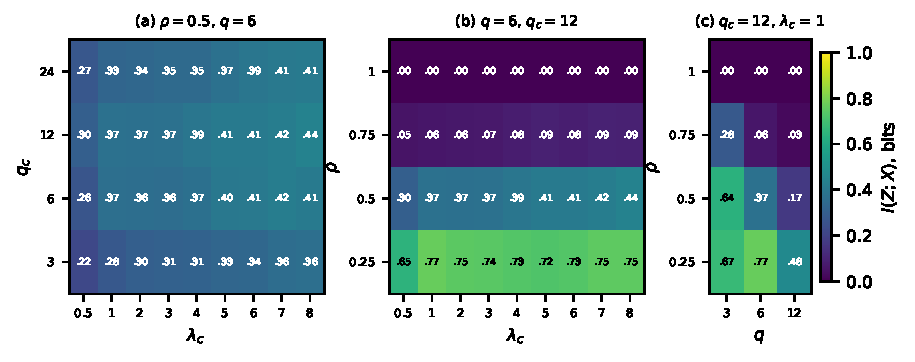
\includegraphics[width=0.98\linewidth]{figures/fig_phase_I_plur.pdf}\\
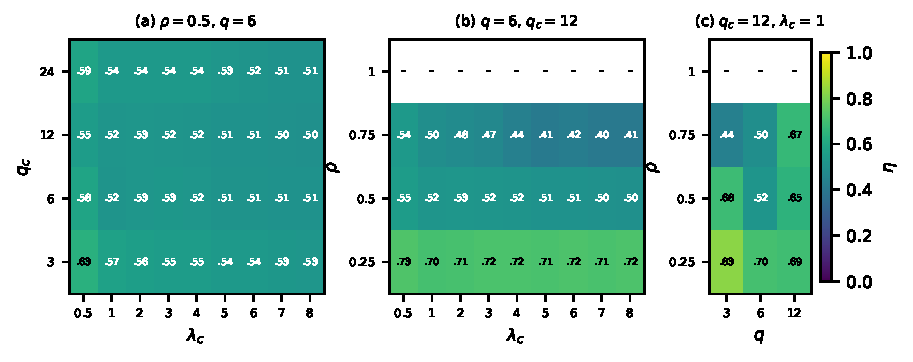
\includegraphics[width=0.98\linewidth]{figures/fig_phase_eta_plur.pdf}
\caption{Readability (top) and efficiency (bottom) at $t = 30$, plurality; panels as in Figure~\ref{fig:phasegain}.}
\label{fig:plurphase}
\end{figure}

\begin{figure}[H]
\centering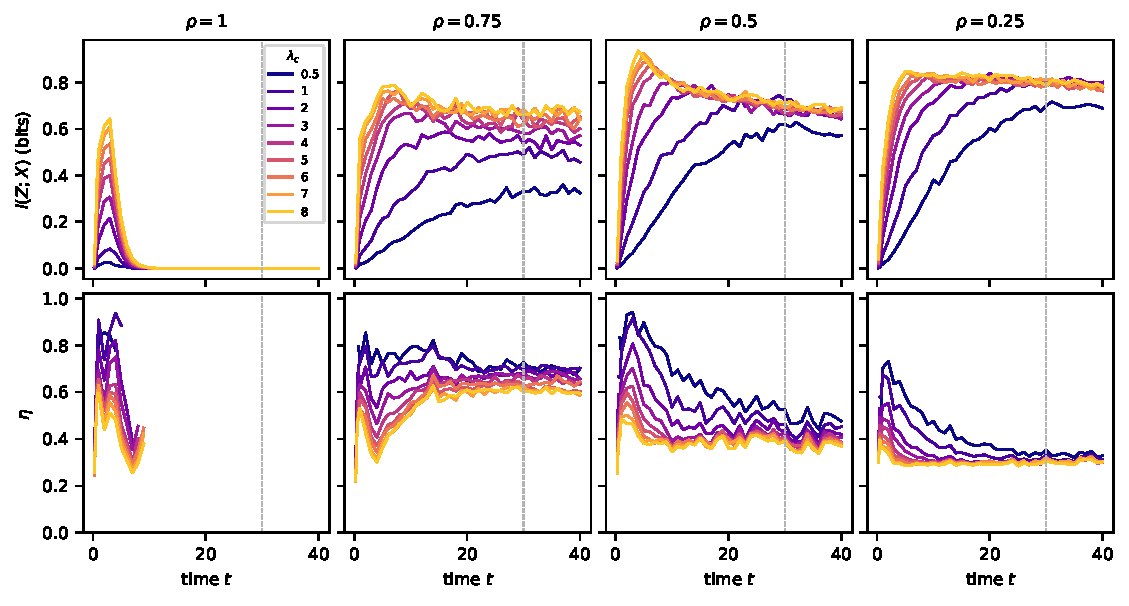
\includegraphics[width=0.95\linewidth]{figures/fig_Ieta_time_s1.pdf}
\caption{As Figure~\ref{fig:plurtime}, with $X$ = S1.}
\label{fig:s1time}
\end{figure}

\begin{figure}[H]
\centering
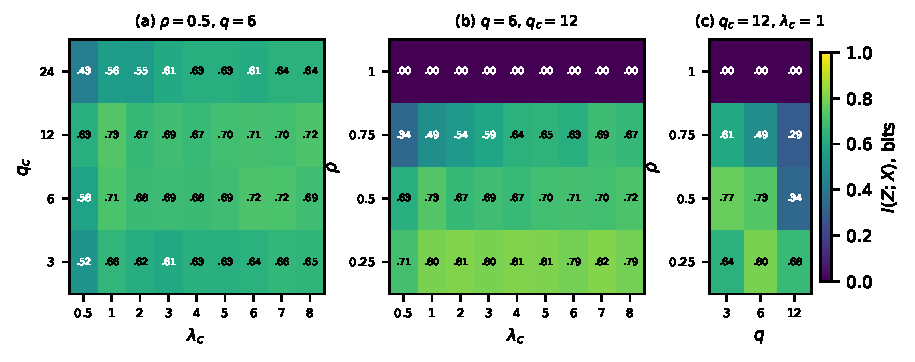
\includegraphics[width=0.98\linewidth]{figures/fig_phase_I_s1.pdf}\\
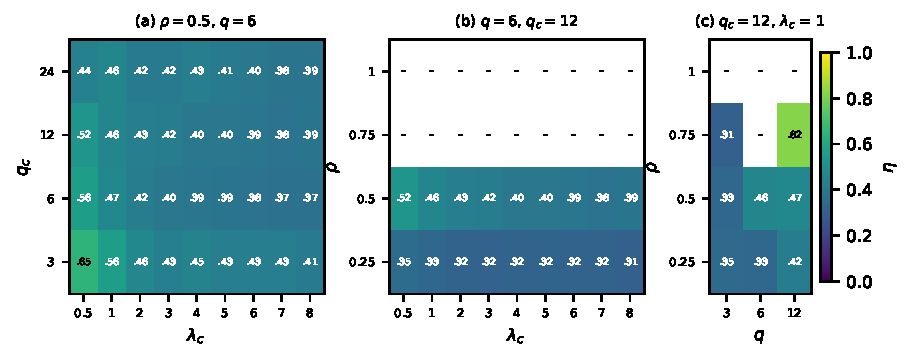
\includegraphics[width=0.98\linewidth]{figures/fig_phase_eta_s1.pdf}
\caption{As Figure~\ref{fig:plurphase}, S1.}
\label{fig:s1phase}
\end{figure}

\begin{figure}[H]
\centering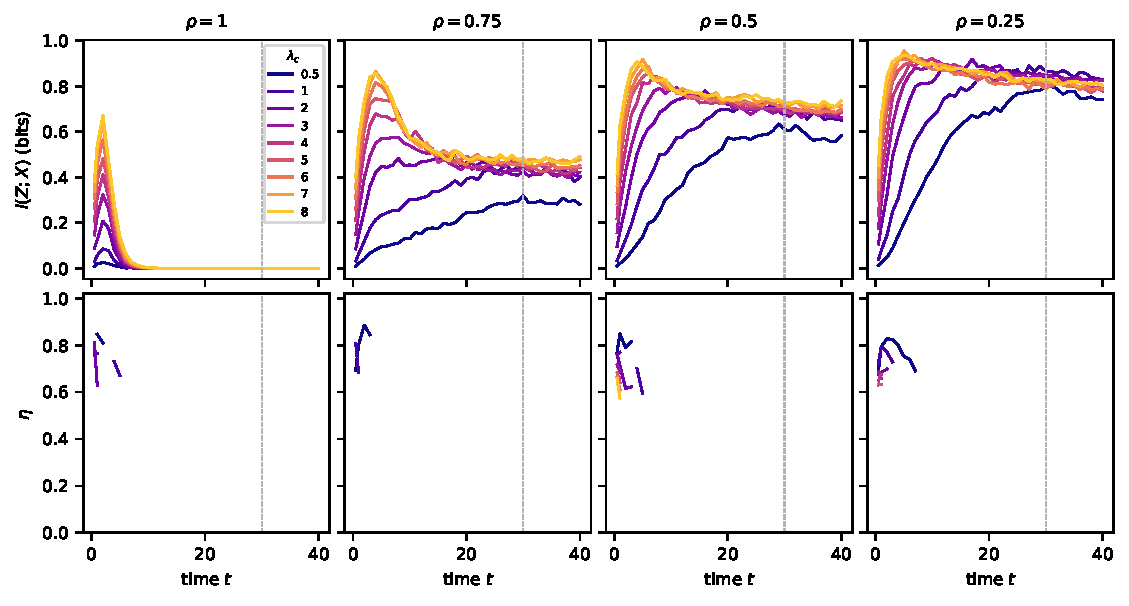
\includegraphics[width=0.95\linewidth]{figures/fig_Ieta_time_s3.pdf}
\caption{As Figure~\ref{fig:plurtime}, with $X$ = S3.}
\label{fig:s3time}
\end{figure}

\begin{figure}[H]
\centering
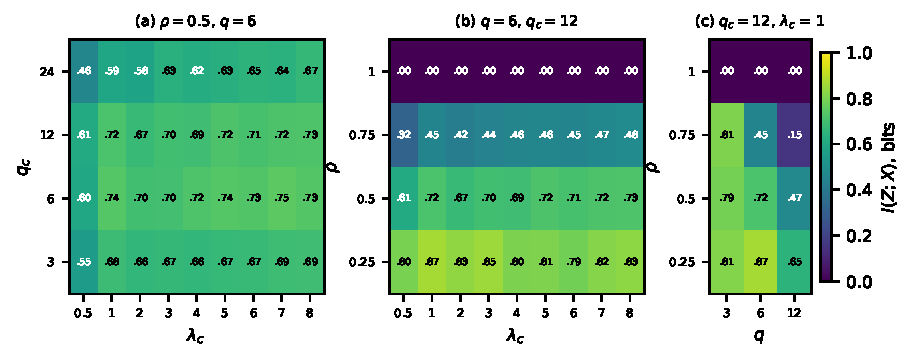
\includegraphics[width=0.98\linewidth]{figures/fig_phase_I_s3.pdf}\\
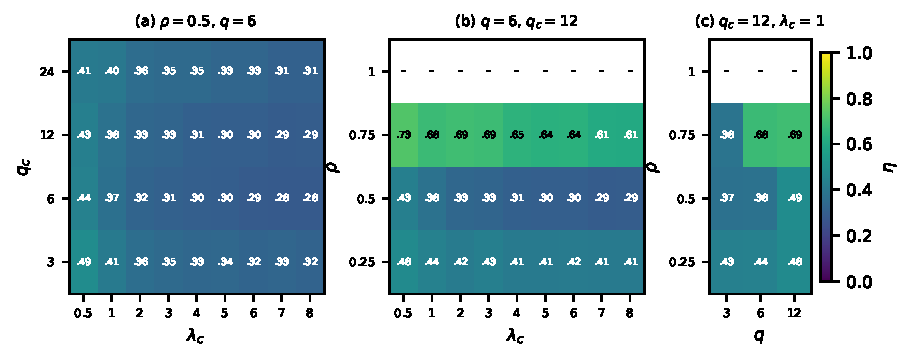
\includegraphics[width=0.98\linewidth]{figures/fig_phase_eta_s3.pdf}
\caption{As Figure~\ref{fig:plurphase}, S3.}
\label{fig:s3phase}
\end{figure}

\begin{itemize}\itemsep1pt
\item \textbf{Swarm-level states read far more than one agent's vote}: at $\rho = 0.25$, $t = 30$, main setting,
  $I = 0.34$ (one vote), $0.76$ (plurality), $0.79$ (S1), $0.86$ (S3) bits; at $\rho = 0.5$, $0.21$, $0.37$,
  $0.72$, $0.71$.
\item \textbf{But their efficiency is lower}: at $t = 30$, main setting, $\eta = 0.49$--$0.70$ (plurality),
  $0.33$--$0.69$ (S1), $0.38$--$0.68$ (S3), against $0.82$--$0.91$ for one vote. Without the pseudo-count of
  Eq.~(\ref{eq:smooth}), $C$ would be infinite for S1 and S3 in many settings (a controlled swarm reaches a bin silence
  never visits). The plurality's $\eta$ is noisier than one vote's because silence rarely lets A2 win (1--18\% of runs),
  so a few episodes set that cell.
\item \textbf{Belief-based states (S1, S3) read the most}, likely because beliefs move before votes do and
  without the noise of the vote draw. The plurality is the swarm state built from votes alone, and its efficiency
  is defined in every setting.
\end{itemize}

\section{Strong control}\label{app:strong}

\begin{figure}[H]
\centering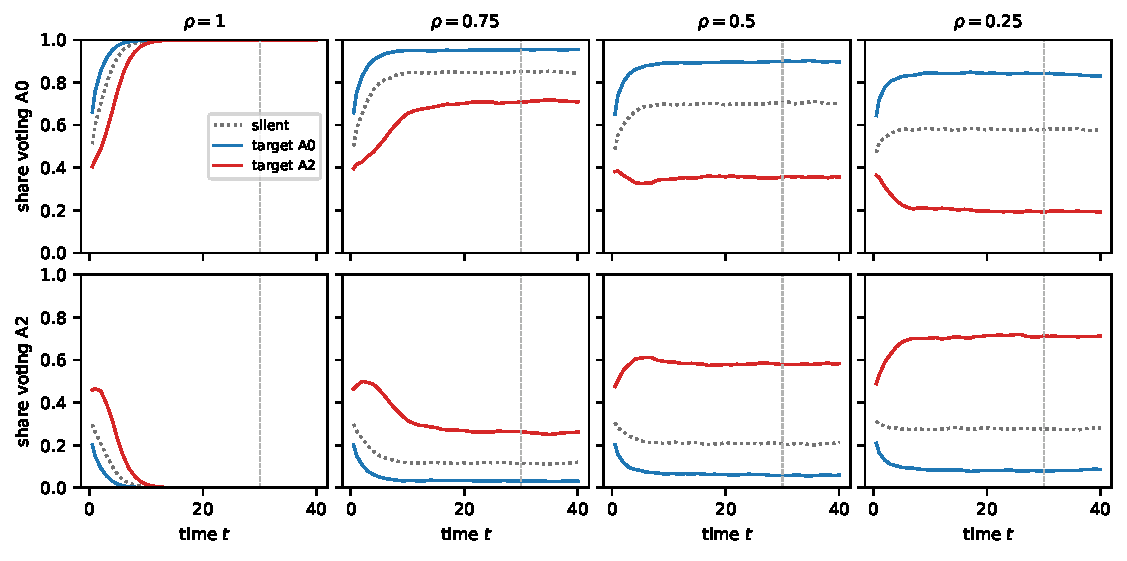
\includegraphics[width=0.95\linewidth]{figures/fig_votes_strong.pdf}
\caption{As Figure~\ref{fig:votes}, at the strongest rate $\lambda_c = 8$.}
\label{fig:votesstrong}
\end{figure}

\begin{figure}[H]
\centering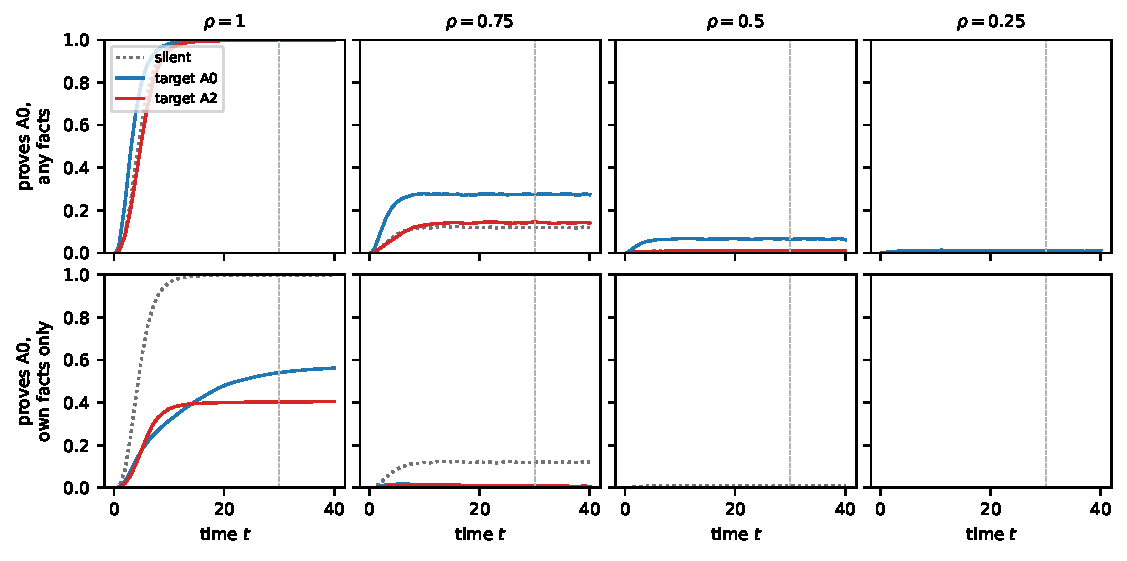
\includegraphics[width=0.95\linewidth]{figures/fig_proofs_strong.pdf}
\caption{As Figure~\ref{fig:proofs}, at $\lambda_c = 8$.}
\label{fig:proofsstrong}
\end{figure}

\begin{itemize}\itemsep1pt
\item \textbf{At $t = 30$ strong control looks like weak control}: target A2 gets 26\%, 58\% and 71\% of votes for
  $\rho = 0.75, 0.5, 0.25$ (23\%, 54\%, 71\% at $\lambda_c = 1$): the 30-message budget, not the rate, sets the end
  point.
\item \textbf{The difference is the path}: a fast controller moves the swarm within a few time units and, at
  $\rho = 0.75$, then loses part of its effect (Figure~\ref{fig:gaintime}).
\item \textbf{Proofs from own facts vanish}: at $\rho = 0.75$, 0.3\% (target A0) and 1\% (target A2) against 12\%
  in silence.
\end{itemize}

\paragraph{Caveats.} One world, 24 exact-Bayesian agents voting by probability matching, one controller policy
with a 30-message budget; 1{,}000 episodes per setting (95\% intervals on $G$ about $\pm0.02$). Information is
plug-in from 1{,}000 episodes per arm. Data:
\texttt{results/simulation\_2/2026-10-15\_sim2\_symmetric\_fine}; tables and figures:
\texttt{analysis/task003\_llm\_free/shared\_analysis/gold\_standard/}.

\end{document}
